Root cause analysis (RCA) is a critical function in operating and managing complex networked systems, be it physical, software, or hybrid~\cite{RCA-Review-2017}.
It aims to identify the component(s) and process(es) responsible for the fault manifested by the wrong results or system failures in a timely fashion.
Traditional RCA relies on accurate system models to deduce the potential component failures from the system symptoms and behaviors.
However,  for large-scale or wide-area networks, the exponential increase of system scales, the complexity of component interdependencies, and the lack of 
visibility into administrative domains have made it impossible to build such models for efficient fault identification and localization. 
As a result, RCA for those systems largely remains a guessing art that requires intensive manual debugging using traditional tools 
like {\it ping} and {\it traceroute} and daunting amount of communication between operators from different organizations 
that often takes days or even weeks.

In order to achieve high availability to support modern distributed applications, automated RCA systems that can quickly identify the root causes of failures 
and performance degradation in much smaller timeframe (minutes for the state-of-art systems) are highly desired for both infrastructure and application service providers. 
In recent years, RCA using machine learning (ML) or data analytic techniques has drawn extensive research and development attention and has found success
 in data center or single domain networks~\cite{netbouncer:nsdi18,Link-JIoT-2019}. Most of these systems aimed to localize the root causes 
 to the particular faulty devices, while some systems focused on coarse-grained classification on the abnormalities either in the server domain or 
 in the network domain~\cite{NetPoirot:Sigcomm2016}. As they are developed for the infrastructure operators, they all have an critical monitoring 
 system like the {\it Ping Mesh}~\cite{guo2015pingmesh} to provide complete topological and measurement information. 

In this paper, we take a different view, an application-centric view, on the RCA system design over a large-scale wide area networked system. 
We specifically use the RCA of data integrity errors for workflow management system (WMS)~\cite{deelman-fgcs-2015}, a popular Internet-scale distributed application, as the use case to 
demonstrate our machine learning based approach. While the challenges and constraints are similar to any other distributed applications, 
we choose WMS mainly because of the inherited flow level measurement capability, broad coverage of the network 
from highly distributed data transfer flows, and access to some limited information about the underneath infrastructure. 
Our basic idea is to formulate the targeted RCA problem as a multi-class classification problem, 
where the potential root causes can be classified based on limited network information and flow level measurements used as training data.  

WMS facilitates in-order execution of jobs in workflows and includes large amounts of interdependent
  data transfers, storage functions, and computation tasks. These tasks are often distributed over distributed hardware, software, and data resources 
  located in different facilities nationwide or globally. Inevitably, frequent system failures and reliability issues 
caused by errors and faults from underlying subsystems have been serious concerns for the WMS community. Since a workflow system is operated as a 
middleware on top of the resources that are managed by different infrastructure service providers (domains), it has no complete knowledge of the health of the infrastructure components, 
the exact topology of the network, and the routing path of the data movement, sometimes even the sources and sinks are abstracted in virtual namespaces. 
Unlike the data center networks, where comprehensive measurement systems can be developed and deployed, like the {\it Ping Mesh}~\cite{guo2015pingmesh}, 
it is not realistic to deploy and operate such a system in the multi-domain wide-area environment to provide necessary network measurement coverage continuously.  

There are other challenges in developing such a RCA system that can achieve high accuracy and low classification time.
 
The first challenge comes from the so-called {\it gray failures} in the networked system. This is in contrast to the so-called {\it hard failures} that will cause data loss or corruption permanently. 
Due to the probabilistic nature of gray failures, the faulty components would act normally most of the time without being caught by existing fault tolerance protocols and monitoring systems. 
Recent studies showed that {\it gray failures} causing performance degradation in terms of packet losses and latency could be efficiently localized using the ML approach~\cite{GrayFailure:2017,DeepView:NSDI18}.  
The data integrity errors, on the other hand, may randomly corrupt bits in a block of data or packets over network transfer. Since existing checksum mechanisms implemented in TCP and the storage services are not 
sufficient to guarantee end-to-end data integrity, they often get unnoticed for a long time until severe consequences to applications occur~\cite{swip:pearc:2019}. Even though the error rate is low, the corrupted  
Modern middleware systems have just started to add end-to-end integrity 
check mechanisms, including in Pegasus~\cite{deelman-fgcs-2015} and Globus~\cite{IntegrityVerification:DataTransfer}. However, root cause localization of integrity errors remains an unsolved problem.

The second challenge lies in the difficulties in acquiring sufficient labeled data to train an ML-based RCA system. Passive monitoring, active probes or event fault injections can be used to generate diagnosis data. However such approaches require substantial investment in developing and operating a comprehensive monitoring system with good coverage, which is more practical for data center networks~\cite{NetPoirot:Sigcomm2016,active:iot:2019}. For Internet-scale system, there is extra limitations in obtaining the accurate network topology and routing information as {\it ping} and {\it traceroute} are always turned off in many domains due to security concerns from the ISP~\cite{topology_obf_20}.

The third challenge is to choose the right ML models to achieve high RCA accuracy out of a large pool of model candidates~\cite{Boutaba:2018aa}. We show that even the most basic questions of defining a data sample, feature selection, and performance evaluation need special consideration. The mixed numerical and categorical features and the imbalanced samples in the multi-class data sets also directly affect the choice of the right ML model.

In~\cite{Link-JIoT-2019}, the authors attempted to identify the hard failures of network links via the popular multi-class ML models using end-to-end passive traffic engineering measurements (throughput, latency, and packet loss). The authors in \cite{DeepView:NSDI18} took an active probe approach to localize the fault in a virtual disk system to the finest granularity up to the network switches. In~\cite{netbouncer:nsdi18}, a necessary condition was derived on the minimal set of paths that active probes need to be sent over the targeted network. Another line of work including~\cite{KDD14,detector:atc17,arzani2018democratically} adapted statistical learning approach to infer the probabilistic relationship between the path failure and the link faults. All these research works made a strong assumption that the RCA system can instrument probes or obtain measurements from any pairs of nodes in the network to obtain both packet-level routing path and measurement information. In an earlier study, the decision tree model was used to predict if a request will succeed over a flawed network system~\cite{DT:2004}. Bayesian inference was demonstrated to be efficient for fast diagnosis when the causal relationship model is established in a large Internet system~\cite{BN-Internet:2007}. A recent study focused on a source based measurement framework to diagnose the issues in the remote application services and therefore does not directly address the network components~\cite{microrca:noms2020}.

\begin{wrapfigure}{ht}{0.26\textwidth}
  \begin{center}
    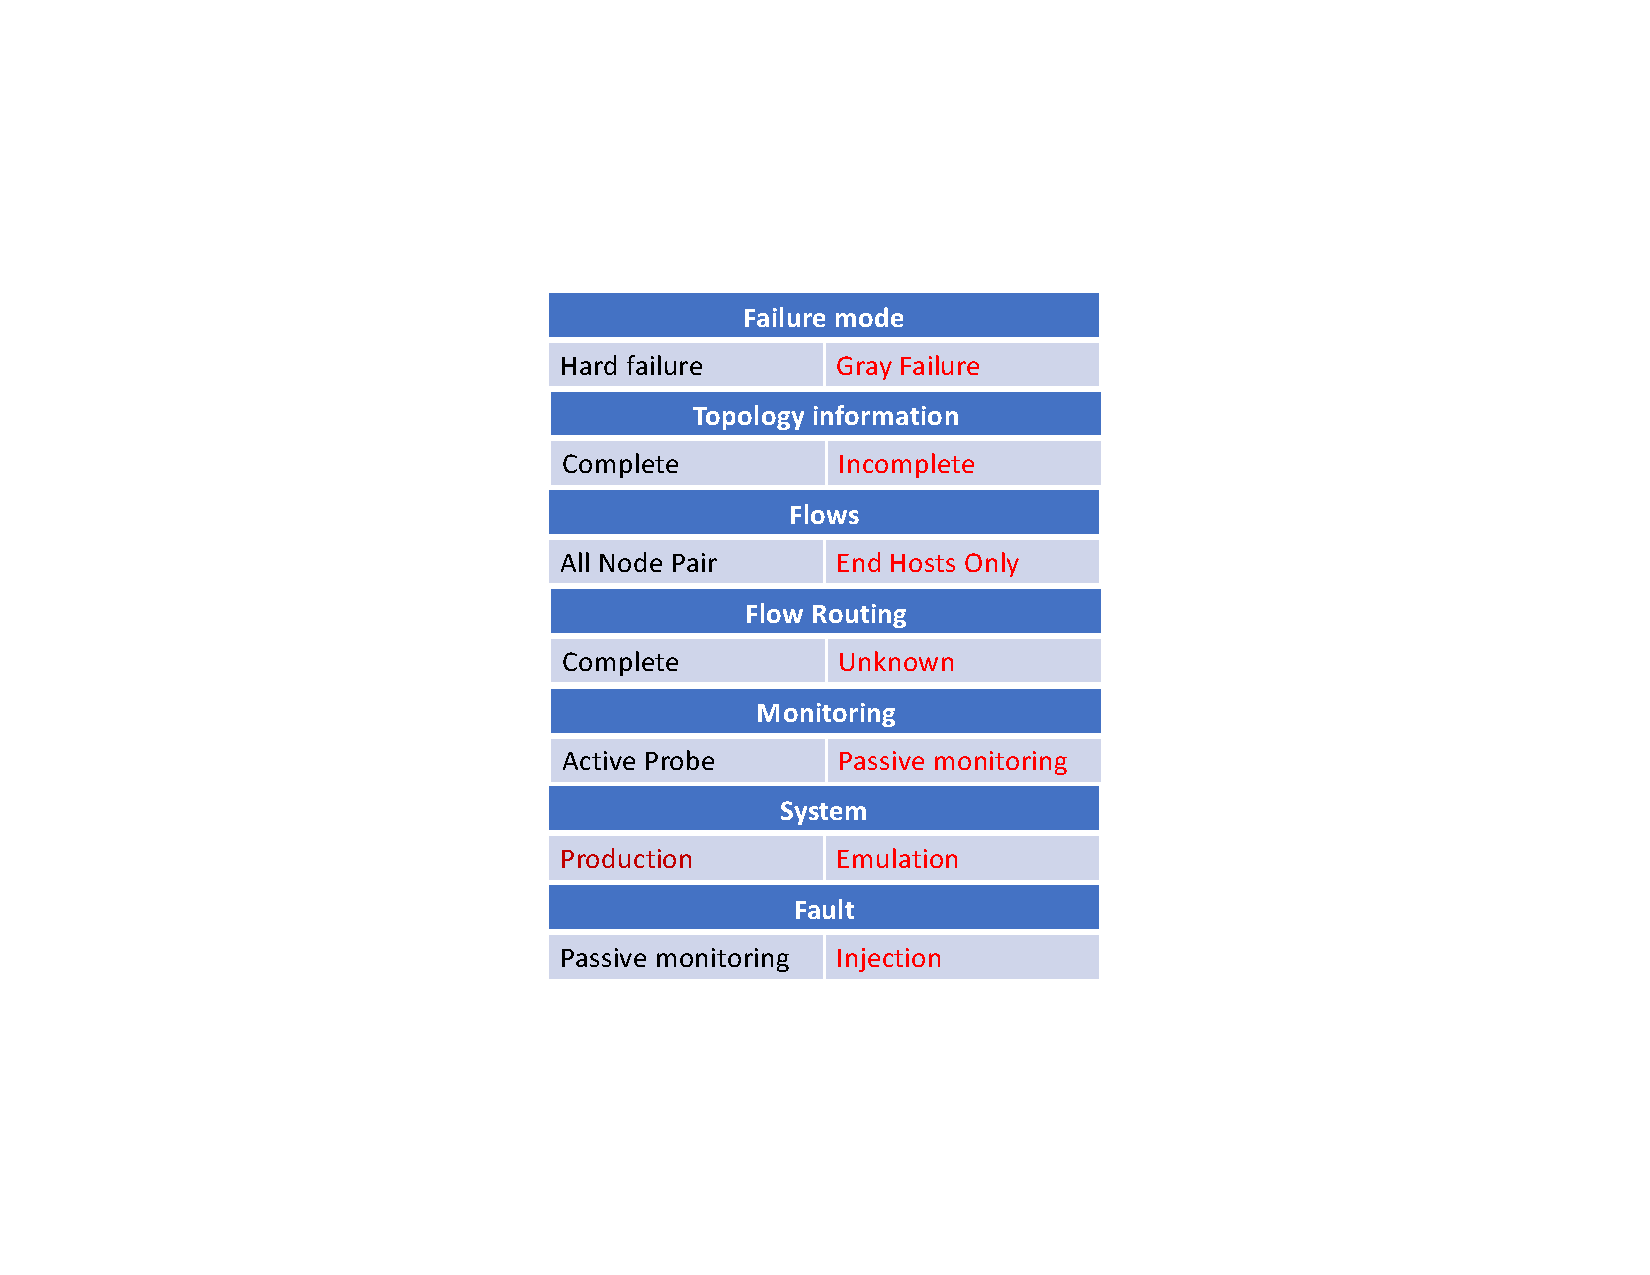
\includegraphics[width=0.26\textwidth]{./figure/RCADesignSpace}
  \end{center}
%  \vspace{-5pt}
\caption{Network RCA Design Space}
%\vspace{-5pt}
\label{fig:designspace}
\end{wrapfigure}

As summarized in Fig.~\ref{fig:designspace}, when developing an efficient RCA system, there are multiple dimensions in the design space. While the majority of recent work in 
gray failure RCA assumed complete network topology and traffic routing knowledge, available system-wide measurement with customized active probing capability in a production 
data center or single domain network, our RCA system falls in the space represented by the right column, which is more adequate and realistic for the Internet scale multi-domain 
environment. Specifically, we assume that only basic network information is available, such as the core routers and all the end hosts in the network. 
Unlike the existing data center RCA systems that often assume active probes being instrumented from any nodes including the routers, 
we assume only passive measurement on the flows between the end hosts is possible from the WMS. In order to obtain sufficient labeled training data and make experiments efficient and repeatable, 
we created a high-fidelity emulation environment in a cloud testbed that can automatically create a virtual network system in virtual machines (VMs), initiate data transfers, inject arbitrary integrity 
errors into the virtual router interfaces and end hosts, and collect training data.

One key motivation underpinning our {\it application-centric} machine learning based approach is to combine the information and capabilities from both application operators and infrastructure operators while not
making unrealistic assumptions beyond domain constraints. If the RCA system can localize the possible failures with high accuracy, the operators of the identified network or end host components can further pinpoint the actual faults within 
a significantly smaller scope, and therefore can lead to fast mitigation or recovery.   

The rest of this paper is organized as follows.We first define the network system integrity error RCA problem with incomplete system and measurement information in Section~\ref{sec:integrity}. We introduce a high-fidelity system emulation environment we created in a cloud testbed in Section~\ref{sec:emulation}. We then present our machine learning approach and model selection in Section~\ref{sec:ml}. We identified that using the network-wide aggregated data flow as the input, training data balancing, and a Top-$k$ accuracy metric can significantly improve the classification accuracy. We evaluated the system performance from the extensive emulation of a representative network in Section~\ref{sec:evaluation}. The impacts of different combinations of numerical and categorical data features under different realistic network and measurement assumptions are quantified. The analysis validated that high RCA accuracy to the device level can be achieved with a random forest model even only partial network and flow level measurement information are available. We conclude the paper in Section~\ref{sec:future}.
